\documentclass[../main/main.tex]{subfiles}

% Put everything that shall appear in the results
% inside this document environment.
\begin{document}
In the following we present several plots showing the results of our experiment evaluations, starting with some information about our demographic data, before displaying general averaged results, followed by a demonstration of individual evaluations of the task performance and bier scores.
\subsection{Demographic Data}
Our questionnaire shown in \ref{appendix:questionaire} has been evaluated on 14 subjects. Their average age was 31.5 years within a range of our youngest 22 year old subject and our oldest subject of 62 years. The group consisted of 6 females and 8 males, all with german nationality and german as their mother language. Their professions included one computer scientist, one scientific coworker, one social worker, one curative educator, one insurance agent and nine students. The subjects of the later included \textit{Psychology in IT} 5 times and \textit{Computer Science} two times. One student's subject was \textit{Social Works}, one was studying \textit{Psychology} and one student came from the field of \textit{Cognitive Science}.
\subsection{Averaged Task Performance and Brier Score}
The average task performance of our subjects is shown in \ref{fig:avg_scores}, with an absolute mean of 2.938 points, averaged across all subjects and tasks, and a standard deviation of 1.391.
\begin{figure}[H]
	\centering
	\captionsetup{justification=centering}
	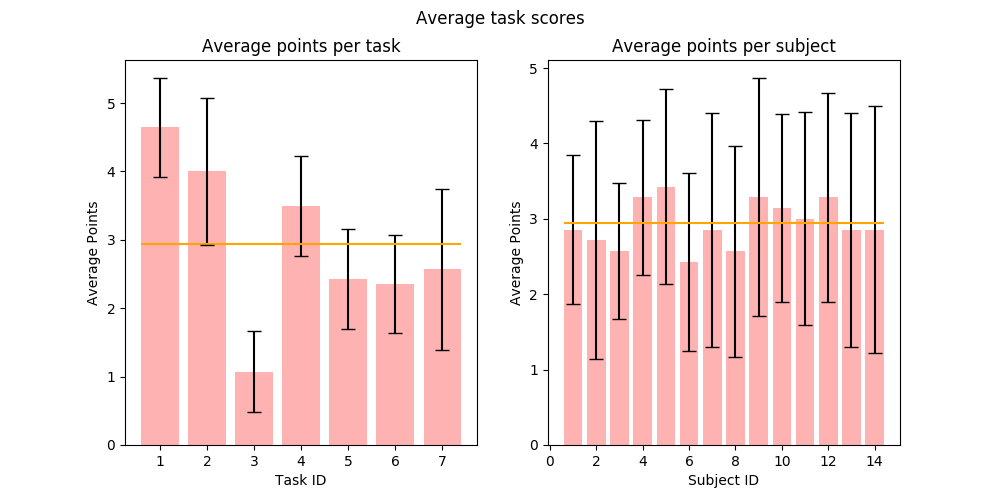
\includegraphics[width=\textwidth]{../assets/average_task_scores.png}
	\caption{Means and standard deviations of the achieved task scores, averaged over subjects in the left and over tasks in the right plot. The orange line displays the overall mean of [TODO], averaged over both variables.]}
	\label{fig:avg_scores}
\end{figure}
The subjects abilities to judge about their own performance, encoded by the average brier score, is displayed in figure \ref{fig:avg_brier} with an overall average of 0.864 and a standard deviation of 0.264. 
\begin{figure}[H]
	\centering
	\captionsetup{justification=centering}
	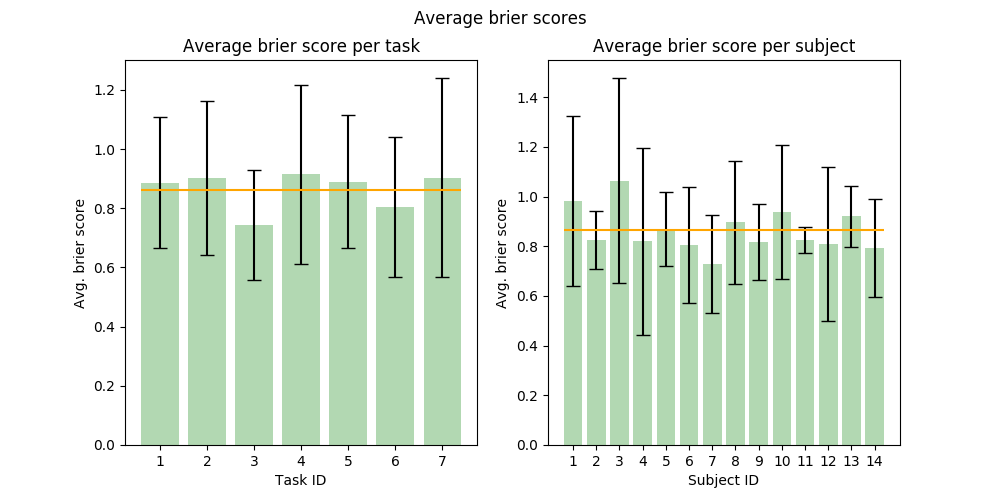
\includegraphics[width=\textwidth]{../assets/average_brier_scores.png}
	\caption{Means and standard deviations of the calculated brier scores, averaged over subjects in the left and over tasks in the right plot. The orange line displays the overall mean of 0.14, averaged over both variables.}
	\label{fig:avg_brier} 
\end{figure}
Please note that we excluded the 8th task from our questionnaire in figure \ref{appendix:questionaire}. For interpretation of these values, please refer to our discussion of the experiment in section \ref{sec:discussion}.
\subsection{Individual Evaluations}
We did individual evaluations of our subjects' task performance, brier scores and confidence ratings. While all figures can be found in appendix \ref{appendix:individual_evaluations}, figure \ref{fig:erhn_results} displays an example for one subject.
\begin{figure}[H]
	\centering
	\captionsetup{justification=centering}
	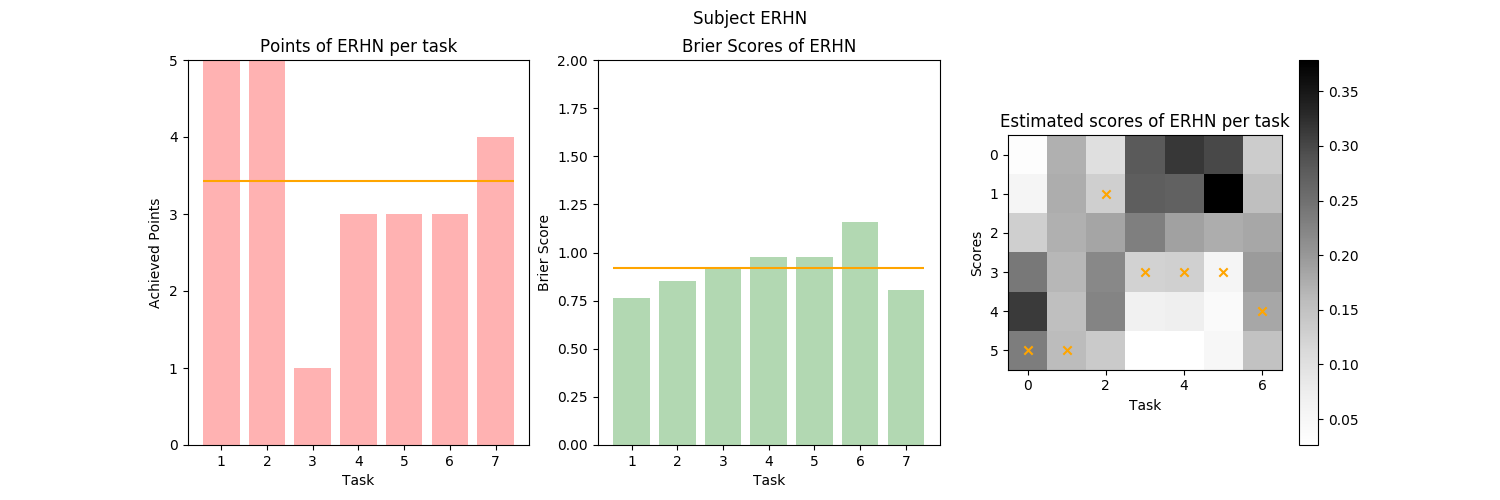
\includegraphics[width=\textwidth]{../assets/ERHN_results.png}
	\caption{Example graphic of our individual evaluations for subject \textit{ERHN}. We again plotted the achieved discrete scores per task on the left and the calculated brier-scores per task in the middle. The orange line displays the mean values for both bar plots, averaged over all tasks. The subject's estimated discrete probabilities of achieving a score are shown in the right graphic, where the orange x marks the actual achieved score in the task. [TODO: FIX X-RANGE OF RIGHT PLOT!]. One could already conclude a tendency of this subject to give underconfident ratings.}
	\label{fig:erhn_results} 
\end{figure}
\subsection{Confidence Plots}
To get more compact insights about our subjects' confidence, we also created scatter plots of the type (Expected Rating) vs (Actual Rating), see figure \ref{fig:erhn_confidence} for an example. A subject's expected rating for a task is calculated out of one column of his or her probability matrix, see the above subsection for an example. The individual plots for all our subjects can be found in appendix \ref{appendix:individual_evaluations}.
\begin{figure}[H]
	\centering
	\captionsetup{justification=centering}
	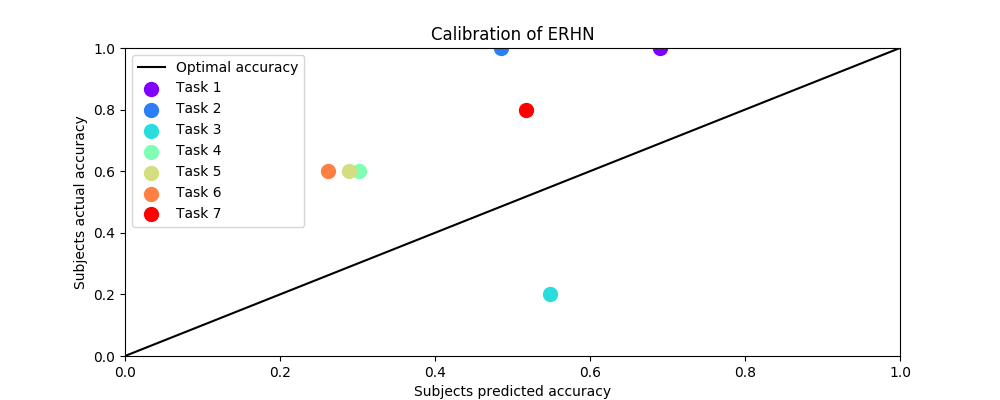
\includegraphics[width=\textwidth]{../assets/ERHN_calibration.png}
	\caption{Example graphic of our individual evaluations on the confidence of subject \textit{ERHN}. We created a scatter plot with the subject's expected rating for each task on the x-axis and his or her actual achieved rating on the y-axis. Optimal confidence is indicated by the solid black line, where expectation meets the actual outcome. Scatter plots of tasks above this line indicate underconfidence for a task, while scatter plots below the line are a sign of overconfidence.}
	\label{fig:erhn_confidence} 
\end{figure}
These average confidence per task is also displayed in figure \ref{fig:avg_confidence}.
\begin{figure}[H]
	\centering
	\captionsetup{justification=centering}
	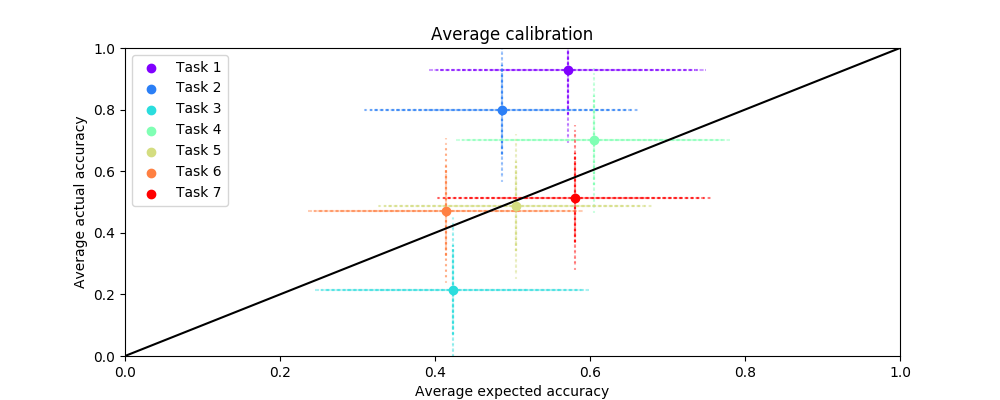
\includegraphics[width=\textwidth]{../assets/average_calibration.png}
	\caption{Scatter plot of average (Expected Rating) vs (Actual Rating) relationship with error bars in both dimensions. Note that the errors are not actual lines around the scores, but the ratings are very likely to be inside the ellipsoids spanned by these standard deviation error bars.}
	\label{fig:avg_confidence} 
\end{figure}
Because we might have found a coincidence between the performance on a task and the confidence of a subject about his rating, we try to get further insights into this by our next evaluation, presented in the next subsection.
\subsection{Task performance vs Brier Score}
To further examine a possible relationship as stated above, we also show the average relationship of (Task Performance) vs (Brier Score) in figure \ref{fig:brier_vs_rating}.
\begin{figure}[H]
	\centering
	\captionsetup{justification=centering}
	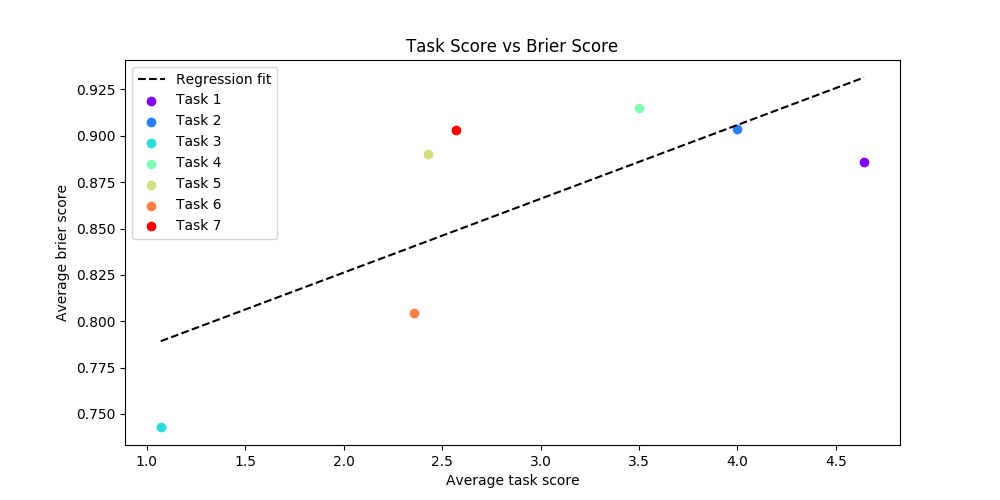
\includegraphics[width=\textwidth]{../assets/brier_vs_rating.png}
	\caption{Scatter plot per task by it's mean task score (x-axis) and it's mean brier score (y-axis), averaged over all subjects. Black dashed line shows a linear regression fit on the data.}
	\label{fig:brier_vs_rating} 
\end{figure}
We also fit a linear regression function on the data, resulting in a seemingly positive correlation between the actual achieved task score and the goodness of the subjects' prediction on it.
\subsection{Overal Estimation}
We also asked our subjects to draw their confidence about the overall performance on the questionnaire. The plots can be found in the filled questionnaires in appendix \ref{appendix:filled_questionaires}, but are not used in our evaluations. The values of these pdfs could be used in further experiments on the topic.\\
We finish with a following discussion about our methods and the presented results in the next section.
\end{document}